%This is chapter 1
%%=========================================
\chapter[Introductions]{Introduction}

This report will review different ...
...\\

%%=========================================
\section{Background}
Norway is among ....... \\


%%=========================================
%\section{Introduction}


%==========================================
\section{Problem Formulation}
Would a ....
\subsubsection{Problems to be addressed}
\begin{itemize}
\item Design ..
\item Develop ...
\end{itemize}

%%=========================================
\section{Literature Survey}
This report is based on ....  published in 2016.
%%=========================================
\section{Objectives}
The Objectives for this report thesis are: 
\begin{enumerate}
\item Make ...
\item Implement ...
\item Create ...
\end{enumerate}

%%=========================================
\section{Scope}
In this particular project .....  

%%=========================================
\section{Structure}
\subsection{Voxelization systems overview}
The diagram in figure \ref{fig:systems-overview} shows how the diffrent software repositories regarding voxelization interconnects. The green boxes represents the main software projects. The blue box represents side projects. During development, some components were generalized and extracted into a separate repository.
\clearpage % remove this ??
\begin{figure}[h]
    \centering
    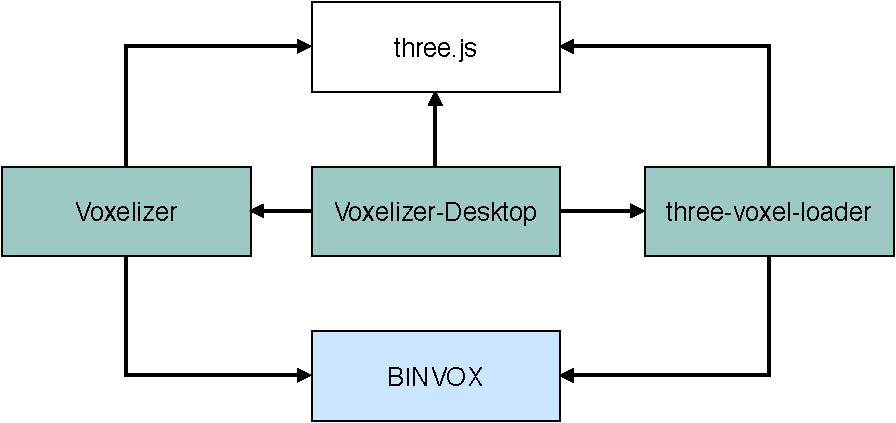
\includegraphics[page=1,scale=1]{sections/introduction/figures/systems-overview.pdf}
    \caption{Automation of release publishing process.}
    \label{fig:systems-overview}
\end{figure}

\subsection{Automation overview}
\colorbox{RubineRed}{Include diagram of simple github automation prosess?}

%%=========================================
\section{Outline}

The rest of the report is structured as follows.\\
\break
\textbf{Chapter 2 - Theory:} Chapter two gives an introduction to the theoretical background .... \\
\break
\textbf{Chapter 3 - Method:} Contains a description of the methodology and materials that were considered throughout the project ....\\
\break
\textbf{Chapter 4 - Result:} Contains a description of the finished software systems \\
\break
\textbf{Chapter 5 - Discussion:} Discusses the achieved results, the execution of methodologies and tools, in addition to encountered difficulties.\\
\break
\textbf{Chapter 6 - Conclusions:} This chapter presents an overall conclusion of the project, reviewing the objectives and the progress made. \\